% This is "sig-alternate.tex" V2.1 April 2013
% This file should be compiled with V2.8 of "sig-alternate.cls" May 2012
%
% This example file demonstrates the use of the 'sig-alternate.cls'
% V2.8 LaTeX2e document class file. It is for those submitting
% articles to ACM Conference Proceedings WHO DO NOT WISH TO
% STRICTLY ADHERE TO THE SIGS (PUBS-BOARD-ENDORSED) STYLE.
% The 'sig-alternate.cls' file will produce a similar-looking,
% albeit, 'tighter' paper resulting in, invariably, fewer pages.
%
% ----------------------------------------------------------------------------------------------------------------
% This .tex file (and associated .cls V2.8) produces:
%       1) The Permission Statement
%       2) The Conference (location) Info information
%       3) The Copyright Line with ACM data
%       4) NO page numbers
%
% as against the acm_proc_article-sp.cls file which
% DOES NOT produce 1) thru' 3) above.
%
% Using 'sig-alternate.cls' you have control, however, from within
% the source .tex file, over both the CopyrightYear
% (defaulted to 200X) and the ACM Copyright Data
% (defaulted to X-XXXXX-XX-X/XX/XX).
% e.g.
% \CopyrightYear{2007} will cause 2007 to appear in the copyright line.
% \crdata{0-12345-67-8/90/12} will cause 0-12345-67-8/90/12 to appear in the copyright line.
%
% ---------------------------------------------------------------------------------------------------------------
% This .tex source is an example which *does* use
% the .bib file (from which the .bbl file % is produced).
% REMEMBER HOWEVER: After having produced the .bbl file,
% and prior to final submission, you *NEED* to 'insert'
% your .bbl file into your source .tex file so as to provide
% ONE 'self-contained' source file.
%
% ================= IF YOU HAVE QUESTIONS =======================
% Questions regarding the SIGS styles, SIGS policies and
% procedures, Conferences etc. should be sent to
% Adrienne Griscti (griscti@acm.org)
%
% Technical questions _only_ to
% Gerald Murray (murray@hq.acm.org)
% ===============================================================
%
% For tracking purposes - this is V2.0 - May 2012

\documentclass{sig-alternate}

%\usepackage[latin1]{inputenc} % Windows
\usepackage[utf8x]{inputenc} % Linux (unicode package needed)
% \usepackage[applemac]{inputenc} % Mac

\usepackage{balance}

\usepackage{graphicx}
\usepackage{caption}
\usepackage{subcaption}
\usepackage{hyperref}

\usepackage{listings}
\usepackage{xcolor}


\colorlet{punct}{red!60!black}
\definecolor{background}{HTML}{FEFEFE}
\definecolor{delim}{RGB}{20,105,176}
\colorlet{numb}{magenta!60!black}

\lstdefinelanguage{json}{
    basicstyle=\small\ttfamily,
    % numbers=left,
    % numberstyle=\scriptsize,
    % stepnumber=1,
    % numbersep=8pt,
    % showstringspaces=false,
    % breaklines=true,
    % frame=lines,
    backgroundcolor=\color{background},
    literate=
     *{0}{{{\color{numb}0}}}{1}
      {1}{{{\color{numb}1}}}{1}
      {2}{{{\color{numb}2}}}{1}
      {3}{{{\color{numb}3}}}{1}
      {4}{{{\color{numb}4}}}{1}
      {5}{{{\color{numb}5}}}{1}
      {6}{{{\color{numb}6}}}{1}
      {7}{{{\color{numb}7}}}{1}
      {8}{{{\color{numb}8}}}{1}
      {9}{{{\color{numb}9}}}{1}
      {:}{{{\color{punct}{:}}}}{1}
      {,}{{{\color{punct}{,}}}}{1}
      {\{}{{{\color{delim}{\{}}}}{1}
      {\}}{{{\color{delim}{\}}}}}{1}
      {[}{{{\color{delim}{[}}}}{1}
      {]}{{{\color{delim}{]}}}}{1},
}

\begin{document}

% Copyright
\setcopyright{acmcopyright}
%\setcopyright{acmlicensed}
%\setcopyright{rightsretained}
%\setcopyright{usgov}
%\setcopyright{usgovmixed}
%\setcopyright{cagov}
%\setcopyright{cagovmixed}


% DOI
\doi{10.475/123_4}

% ISBN
\isbn{123-4567-24-567/08/06}

%Conference
\conferenceinfo{DocEng2015}{Sep 8--11, 2015, Lausanne, Switzerland}

\acmPrice{\$15.00}

\title{HIJSON: a cartographic document format for web modeling 
of interactive indoor mapping}


\numberofauthors{6}
\author{
\alignauthor
Marco Virgadamo\\
 \affaddr{Dipartimento di Ingegneria}\\
 \affaddr{Universit\`a Roma Tre}\\
 \affaddr{Rome, Italy}\\
 \email{virgadamo@dia.uniroma3.it}
\alignauthor
Marco Sportillo\\
 \affaddr{Dipartimento di Ingegneria}\\
 \affaddr{Universit\`a Roma Tre}\\
 \affaddr{Rome, Italy}\\
 \email{sportillo@dia.uniroma3.it}
\alignauthor 
Federico Spini\\
 \affaddr{Dipartimento di Ingegneria}\\
 \affaddr{Universit\`a Roma Tre}\\
 \affaddr{Rome, Italy}\\
 \email{spini@dia.uniroma3.it}
\and % use '\and' if you need 'another row' of author names
\alignauthor 
Alberto Paoluzzi\\
 \affaddr{Dip. di Matematica e Fisica}\\
 \affaddr{Universit\`a Roma Tre}\\
 \affaddr{Rome, Italy}\\
 \email{paoluzzi@dia.uniroma3.it}
\alignauthor 
Enrico Marino\\
 \affaddr{Dipartimento di Ingegneria}\\
 \affaddr{Universit\`a Roma Tre}\\
 \affaddr{Rome, Italy}\\
 \email{marino@dia.uniroma3.it}
\alignauthor 
Antonio Bottaro\\
 \affaddr{Sogei S.p.A.}\\
 \affaddr{Ricerca e Sviluppo}\\
 \affaddr{Rome, Italy}\\
 \email{abottaro@sogei.it}
}

\date{23 March 2015}

\maketitle

\begin{abstract}

This paper introduces HIJSON\footnote{This work was partially funded with
grants by Sogei S.p.A.,the ICT company of the Italian Ministry of Economy and
Finance.}, a novel indoor cartographic document format. A software framework
is also presented, that relies on HIJSON documents and is entirely based on
web technologies. With respect to current cartographic formats, HIJSON brings
four major enhancements: (a) exposes a hierarchical structure; (b) uses local
metric coordinate systems; (c) may import external geometric models; (d)
accepts semantic extensions. The HIJSON format is designed to describe any
geometry of the \emph{indoor space} of complex buildings, capturing their
hierarchical structure, a complete representation of their topology, and all
the objects (either smart or not) contained inside. The textual representation
allows the software framework to offer a web environment in which the user is
presented with either 2D or 3D models of the indoor ambient to navigate. Such
virtually rebuilt environment, accessible via web browsers from any kind of
device, can be regarded as the platform where several applications may
coexist: IoT monitoring; realtime multi-person tracking; cross-storey user
navigation, through an algorithm that automatically finds valid walkable
routes, taking into account both architectural obstacles and furniture. The
semantic extensions supported by the HIJSON framework architecture encapsulate
the details about communication protocols, rendering style, and exchanged and
displayed information, allowing the HIJSON format to be extended with any sort
of models of objects, sensors or behaviors.

\end{abstract}


%
% The code below should be generated by the tool at
% http://dl.acm.org/ccs.cfm
% Please copy and paste the code instead of the example below. 
%

\begin{CCSXML}
<ccs2012>
<concept>
<concept_id>10002951.10003260.10003282</concept_id>
<concept_desc>Information systems~Web applications</concept_desc>
<concept_significance>500</concept_significance>
</concept>
<concept>
<concept_id>10010405.10010476.10010479</concept_id>
<concept_desc>Applied computing~Cartography</concept_desc>
<concept_significance>500</concept_significance>
</concept>
<concept>
<concept_id>10010405.10010497.10010510.10010514</concept_id>
<concept_desc>Applied computing~Format and notation</concept_desc>
<concept_significance>500</concept_significance>
</concept>
<concept>
<concept_id>10010520.10010521.10010537.10010538</concept_id>
<concept_desc>Computer systems organization~Client-server architectures</concept_desc>
<concept_significance>300</concept_significance>
</concept>
<concept>
<concept_id>10010520.10010570.10010574</concept_id>
<concept_desc>Computer systems organization~Real-time system architecture</concept_desc>
<concept_significance>300</concept_significance>
</concept>
</ccs2012>
\end{CCSXML}

\ccsdesc[500]{Information systems~Web applications}
\ccsdesc[500]{Applied computing~Cartography}
\ccsdesc[500]{Applied computing~Format and notation}
\ccsdesc[300]{Computer systems organization~Client-server architectures}
\ccsdesc[300]{Computer systems organization~Real-time system architecture}

%
% End generated code
%

%
%  Use this command to print the description
%
\printccsdesc

% We no longer use \terms command
%\terms{Algorithms, Design, Documentation, Standardization}

\keywords{Document format, indoor cartography, indoor navigation, IoT monitoring, HIJSON, multiperson tracking, web 3D, web cartography}

\section{Introduction}\label{introduction}


Among the many activities of R\&D Sogei, we are now analyzing the
computingofposition data during the transition between outdoor and
indoorscenarios. In orderto achieve our purpose we are experimenting
severaltechnologies, such asGNSS (Global Navigation Satellite system), WI­FI,
LTE(Long Term Evolution),SDR(Software Defined Radio). 






We are now trying to
verify the possibility to perform a realtime control over the maintenance
workflow in a complex Data Center. 


Inparticular, wehave to support the process of those in charge of carrying out the ticket­maintenance reaching, as quick as possible and without error, the right sub­system
(inside the rightrack among thousands). We will call them the ‘maintenance man’. The real­time awareness of the relative positions between the ‘maintenance man' andthe rack ­ containing
the sub­system ­ will help us reducing intervention times and increasing safety.
If you knew when the maintenance process starts, you couldautomatically
move,in real time, services, that is virtual machines, to other systems,thus
maintainingcontinuity of services and, in the same time, reducing the
globalrisk factor. Whenmaintenance is over, and the technician moves away, you
couldinstantly restore thepre­existing conditions of services, that is,
immediately after havingperformed anoutright test.



VASTI AMBIENTI 



MOLTI SENSORI E SISTEMI DI RILEVAZIONE DELLA POSIZIONE DIFFERENTI

CONTINUOUS OUTDOOR-INDOOR NAVIGATION


MONITORAGGIO DI SCENARI UNIFICATI DI INTERVENTO UOMO MACCHINA


PERSONALE TECNICO DEVE ESSERE GUIDATO 



IL PASSAGGIO DA SERVER A IOT È IMMEDIATO


MONITORAGGIO UNIFICATO DEGLI SMART OBJECTS IOT






SERVER REAL MACHINE (that can be assimialted to smart objects in the IoT context, since )






DESCRIZIONE DELLE PROBLEMATICHE 

TALI PROBLEMATICHE SONO TIPICHE DI SCENARI IN CUI SIA NECESSARIO IL CONTROLLO DEGLI ACCESSI
LA SUPERVISIONE, ...






IN QUESTO SCENARIO SI PONE IL LAVORO DESCRITTO IN QUESTO PAPER, 
IN CUI LE NECESSIT`A DESCRITTE VENGONO AFFRONTATE PARTENDO DALLE BASI,
OVVERO DEFINENDO UN FORMATO DI DOCUMENTO PER LA DESCRIZIONE ASTRATTA DI AMBIENTI INDOOR.
DESCRITTO L'AMBIENTE DEVE QUINDI ESSERE POSSIBILE RICOSTRUIRE VIRTUALMENTE L'AMBIENTE
RENDERLO LARGAMENTE ACCESSIBILE VIA WEB, E MONTARE SU QUESTA RAPPRESENTAZIONE VIRTUALE 
LA POSSIBILIT`A DI INTERAGIRE CON GLI OGGETTI ALL'INTERNO DELL'AMBIENTE. L'INTERAZIONE DEVE CONSISTERE DA UN LATO NALLA POSSIBILIT`A DI RICEVERE INFORMAZIONI DALL'OGGETTO, MA ANCHE DI INVIARE COMANDI ALL'OGGETTP.

SI REALIZZA IN QUESTO MODO UNO SCENARIO IN CUI UN SUPERVISORE INTERAGISCE CON L'AMBIENTE IN CUI SI MUOVE UN EXPLORER (O MANUTENTORE) POTENDO IL SUPERVISORE AVERE IMMEDIATA NOTIFICA DELLA POSIZIONE DEL MANUTENTORE, E AVENDO UN QUADRO COMPLETO FORNITO DAGLI OGGETTI SMART PRESENTI NELL'AMBIENTE REALE ASSIEME ALL'EXPLORER.

D'ALTRA PARTE PER GRANDI SPAZI ANCHE L'EXPLORER PUO ESSERE SUPPORTATO DAL SISTEMA CHE AVENDO COMPLETA CONOSCENZA DELLA TOPOLOGIA E DELLA GEOMETRIA DELL'AMBIENTE, NONCHE DEGLI OGGETTI IN ESSO CONTENUTI, POSSIEDE TUTTE LE INFORMAZIONI NECESSARIE PER GUIDARE L'EXPLORER ATTRAVERSO L'AMBIENTE.

NULLA IMPEDISCE DI MIXARE LE NECESSITÀ DI EXPLORER E SUPERVISOR, REALIZZANDO UN EXPLORER CHE NAVIGA NELL'AMBIENTE REALE ED IN ESSO RICEVE INFORMAZIONE E A CONTEMPO PUÒ INVIARE COMANDI AGLI SMART OBJECT INTORNO A SE.

\ldots{}

The remainder of this document is organized as follows. In Section II is
provided an overview of the state of the art in the field of indoor document
standard and related applications. Section III is devoted to describe the
advances introduced by the novel cartographic document proposed, while section
IV presents the document syntax. Section V reports about the toolkit
specifically developed to handle the new document format. In Section VI is
depicted the overall architecture and the implementation of the web based
application framework, which is in turn used to achieve the objectives stated above.
Finally, Section VII proposes some conclusive remarks and future developments.


\section{Related work}\label{related-work}

Researches about the cartographic representation of indoor environments are
numerous and at the same time heterogeneos regarding to the strategies
applied. Different information sources are used, and accuracy of the
produced solution depends on the adopted approach. In some cases the
information is obtained with automatic or semi-automatic processing of files
that describe the architectural structure of a building, such as BIM (Building Information Modeling)~\cite{Eastman:2008:BHG:1796500} and/or IFC (Industry Foundation Classes) that describe a building project \cite{6816739}. Image processing is also used to
extract topological information from floor plan images \cite{6878152}. In
other works, building informations and descriptive parameters are redefined
from scratch \cite{6418876}. This choice is driven by the unsuitableness of
the current representive formats: images contain poor information and CAD
files are not designed for this kind of use. 

A recurring theme among the use
of carthograhic information is \emph{indoor navigation}
\cite{6878152,6418876,6816739}. The proposed approaches are very different in
this case too, and based on several strategies with some basic elements in
common. An often adopted solution is based on the representation of the
routing information as a graph, having a node for each room and an edge for
each couple of connected rooms. In some cases the edges are weighted in
function of euclidean distance. The detail level of the graph and hence the
effective practicalbility of the calculated paths, can vary depending on the
technique and the design choices applied, but in general most of the proposed
solutions retrieve information only from architectual structure. 

A subject related to navigation is the \emph{location of users}. All the considered works
agree on the inadequacy of GNSS in indoors contexts, due to the segnificant
reduction in signal quality. To locate the exact position of a user inside a
building, the currently most used techniques are based on fingerprinting and
triangulation of radio signals (WiFi, Bluetooth, etc.) flanked by more
original solutions based on, for example, image recognition \cite{6815564}.
User tracking issue is faced with solutions that range from the clever
utilization of inertial tracking sensors embedded in many smartphones
\cite{6815564} to the adoption of ad hoc devices \cite{6878152}.

The actual ``de-facto'' standard in terms of geospatial data representation is
the GeoJSON format, which can be easily used for any type of geographical
annotation. In some cases it has been slightly adapted to be used in indoor
environments (IndoorJSON).

\subsection{The GeoJSON format}\label{the-geojson-format}

GeoJSON is a geospatial data interchange format based on JSON, suitable for a
geometrical encoding of various geographic data structures. As opposed to GIS
format, GeoJSON is an open standard. Positions need to be expressed in
geographical coordinates (usually WGS84).

GeoJSON supports some geometric primitives, including: \texttt{Point},
\texttt{Line\-String}, \texttt{Polygon}, \texttt{MultiPoint},
\texttt{MultiLineString}, and \texttt{MultiPolygon}. Lists of geometries are
represented by a \texttt{GeometryCollection}. Geometries with additional
properties are \texttt{Feature} objects. Lists of \texttt{Feature} are
represented by a \texttt{FeatureCollection}.

A single \texttt{Feature} is composed essentially by two mandatory fields:
\texttt{geometry}, which describes the objects' geometry accordingly to the
previously defined primitives, and \texttt{properties} which contains
additional information about the \texttt{Feature}.

It is possible to define complex shapes through the composition of simple
GeoJSON objects. Mainly due to its semplicity, GeoJSON is widely used and
deeply integrated in several applications and services.

\subsection{The IndoorJSON format}\label{experiences-on-indoor-json}

IndoorJSON is a GeoJSON variant defined and used by \emph{indoor.io}, a
Finnish company devoted to indoor environment mapping. IndoorJSON is compliant
with GeoJSON syntax, and it may consist of any number of \texttt{Features}
and/or \texttt{FeatureCollections}. All \texttt{Features} are interpreted
similarly regardless of their grouping into nested
\texttt{FeatureCollections}. IndoorJSON supports all GeoJSON geometry types.

Some particular properties are used to correctly define indoor elements:

\begin{itemize}
\itemsep1pt\parskip0pt\parsep0pt
\item
 \texttt{level}: described which level contains the feature;
\item
 \texttt{geomType}: identifies the object's
 category, useful during the visualization
 process.
\end{itemize}

There are some additional not mandatories properties useful for
the indoor representation:

\begin{itemize}
\itemsep1pt\parskip0pt\parsep0pt
\item
 \texttt{accessible}: describes if an element is walkable or not;
\item
 \texttt{connector}: defines if the element is a connection between two
 levels;
\item
 \texttt{direction}: describes the direction of the connection (both
 ways, only up, only down);
\end{itemize}

A syntax validator is provided by \emph{indoor.io}, but the commercial nature
of this project limits the number of tools available to deal with this
format.



\section{Advances on cartographic\\ document formats}\label{advances-on-cartographic-document-format}
\label{advances}

The focus of this work is the definition of a novel format of cartographic
documents along with the software ecosystem rooted on it. A simple but
effective algorithm to find indoor valid routes is also provided. The {HIJSON}
(\textbf{H}ierarchical \textbf{I}ndoor \textbf{JSON}, this is the name chosen
for the format) and the accompanying software framework aim to realize a
mapping of indoor real spaces with a virtual interactive web environment. The
HIJSON is based upon ideas and design principles collected from previous
formats and identifies four critical improvements with respect to them: it
exposes a \emph{hierarchical structure}, uses \emph{metric local coordinate
system} \emph{imports external hyperlinked geometric models} and accepts \emph{semantic
extensions}. 
% Furthermore, geometrical  and topological data are conveniently imported and represented via LAR, an advanced  representation scheme, allowing to deal with \emph{hyperlinked geometric models}.

\subsection{Hierarchical structure}\label{hierarchical-structure}

The HIJSON format allows for hierarchical description of indoor spaces. The
introduction of a hierarchical structure establishes a parent-child relation
between entities of the model, reflecting a container-contained relationship.
This direclty implies a neater representation than the plain linear structure
adopted by GeoJSON, being a perfect analogy of objects contained (i.e.
placed) into spaces.

In addition, more organized arrangement is allowed by logical (or even
physical) grouping: concepts like building wings, sections, stories,
departemens, etc. can be introduced to reflect into the document structure
logical or physical real divisions, categories or relashionships.

Hierarchical structures are common in computer graphics since they are used as
scenegraphs. This accordance of underlying structures really simplify 3D
render algorithms of HIJSON documented environments.

Furthermore the container-contained relation enables to use local reference system.

\subsection{Metric local coordinate system}\label{metric-local-coordinate-system}

Supported by the hierarchical underlying structure, the HJSON document format allows 
for the use of local coordinate system. This means that the shape of all elements can 
be convenient modelled using local coordinate and than placed in the right position 
with respect to the position of the parent (or container) element applying a 
translation and a rotation vector.

Another substantial advantage is represented by the adoption of a metric reference, 
consequently simplifying the compilation of the document, however it is, 
manual or aided by software tools.

The HIJSON document format is specially designed to guarantee the user to be routed seamlessly 
from outdoor to indoor and vice versa. Even though indoor geometries are inputted in a metric 
local continuous outdoor-indoor navigation is ensured via the definition of a processing pipeline
detailed in the following.

\subsection{Hyperlinked geometric models}\label{optional-lar}

A HIJSON document may further import external geometric models---either of the buildings itself or the interior furniture or devices---that are topologically complete (in the sense of solid modeling~\cite{Requicha:1980:RRS:356827.356833}) and very compact. 
Such models coming from a source outside the document are acquired by linking JSON files that contain a Linear Algebraic Representation (LAR) of topology and geometry, to be expanded for visualization or interaction at any useful level of detail. 

The LAR scheme~\cite{Dicarlo:2014:TNL:2543138.2543294} is characterised by a very large domain, including architecture, building and construction~\cite{paoluzziMS:2014}, 2D and 3D engineering meshes, non-manifold geometric and solid models and meshes, and high-resolution 3D images~\cite{cadanda:2015}. This scheme uses the set of \emph{Combinatorial Cellular Complexes} (CCC) as mathematical domain
\cite{Basak:2010}, and various compressed representations of \emph{sparse matrices} \cite{gemmexp} as codomain. 

Since LAR provides a complete representation of the topology of the represented space,
the matrix $[\partial_d]$ of the boundary operator shall be used to compute the coordinate representation $[c]$ of the \emph{boundary} chain of \emph{any subset} $c$ of cells, though \emph{a single} operation of SpMV multiplication \cite{gemmexp} between the \texttt{CSR} (Compressed Sparse Row) representation of $[\partial]$ and the \texttt{CSC} (Compressed Sparse Column) representation of the $[c]$ chain, resulting in very efficient computations on modern hardware, even mobile.

The expansion of a LAR model, to be considered as a general-purpose graphic primitive, may be executed on either the server or the supervisor client of the HIJSON Web Toolkit architecture (see Section~\ref{server-architecture}), or even on the \emph{Explorer} client, depending on the size and the locality of the model to be expanded.

% \begin{figure}[htbp] % figure placement: here, top, bottom, or page
% \centering
% 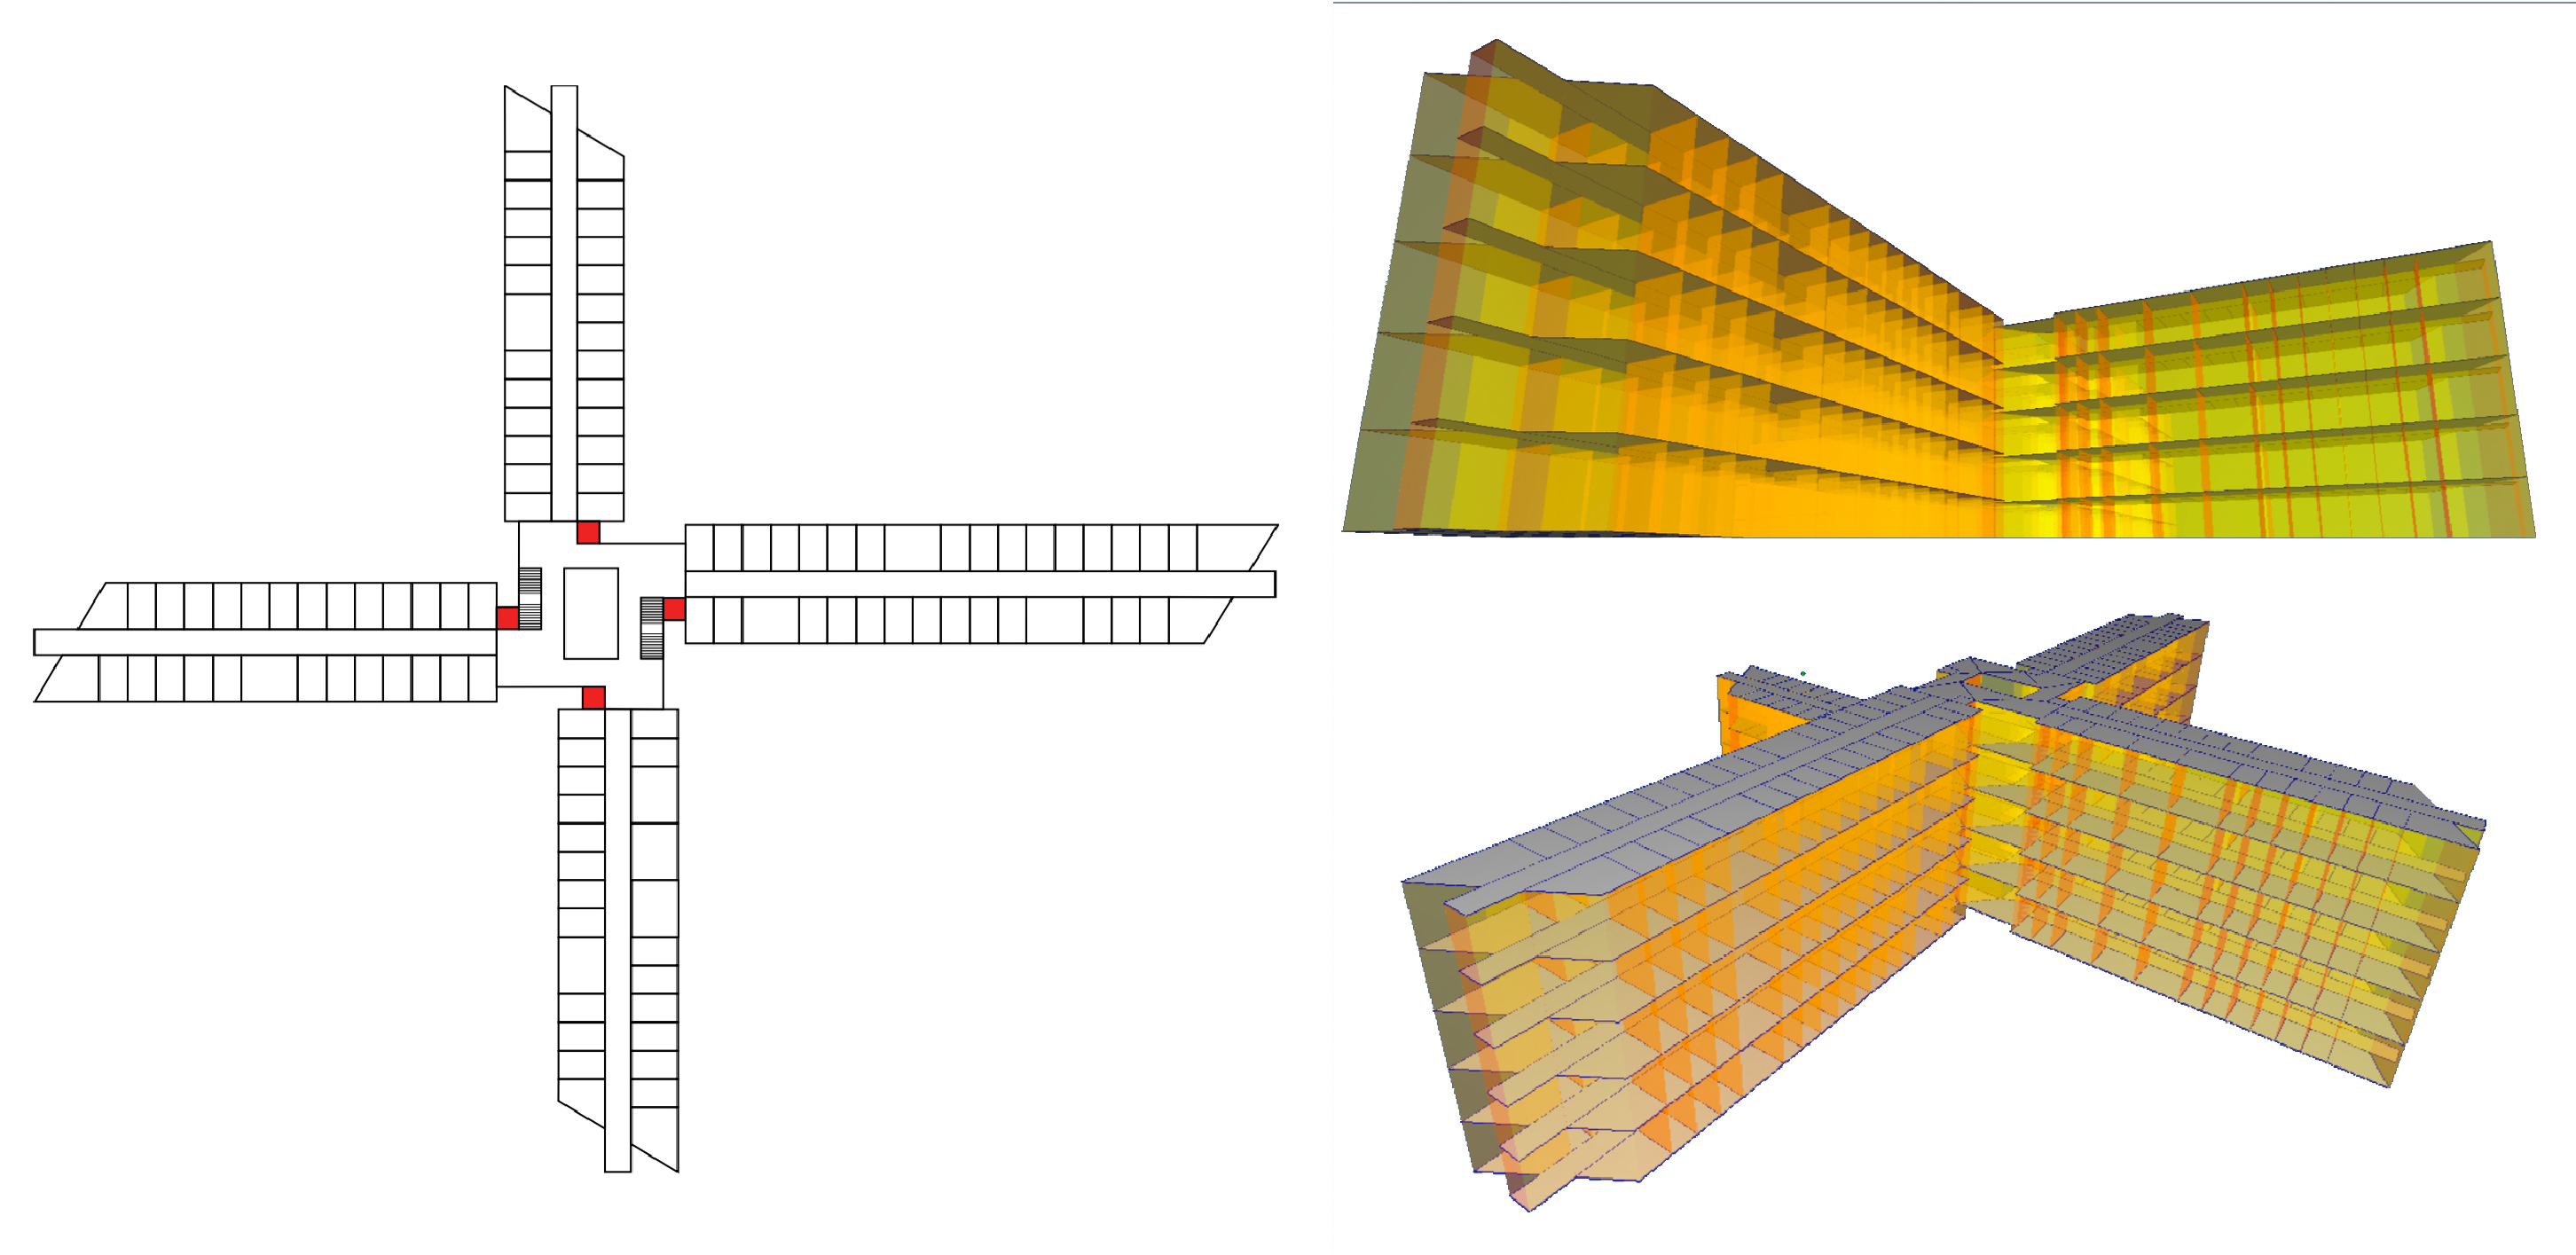
\includegraphics[width=\linewidth]{images/sogei} 
% \caption{Office building: (a) the schematic plan; (b) the simplified 3D model generated for testing on the field the in-door mapping project described in this paper.}
% \label{fig:sogei}
% \end{figure}

\begin{figure}[!h]
 \centering
 \begin{subfigure}[b]{0.48\linewidth}
 \includegraphics[width=\textwidth]{images/sogei-a} 
 \caption{}
 \label{fig:sogei-a}
 \end{subfigure}
 ~
 \begin{subfigure}[b]{0.48\linewidth}
 \includegraphics[width=\textwidth]{images/sogei-b}
 \caption{}
 \label{fig:sogei-b}
 \end{subfigure}
 
 \caption{Office building: 
 (a) the schematic plan; 
 (b) the simplified 3D model generated for testing on the field 
 the in-door mapping project described in this paper.
 }
 \label{fig:sogei}
\end{figure}

\subsection{Semantic extensions}\label{semantic-extensions}

Semantic extensions make the HIJSON format extendible and customizable, that
is, able to adequately respond to any need of objects representation. To define a
semantic extension means to allow the HIJSON document to model an object
previously not covered, or even to modify the behaviour of a comprised one.
Semantic extensions are to be defined both as HIJSON format syntyax and as
HIJSON Toolk source code. In particular it is necessary to define respectively
a new HIJSON Element and a new HIJSON Class, as specified below.




\section{HIJSON structure and syntax}\label{hijson-syntax}

In listing~\ref{lst:hijson-example} it is shown a simplified HIJSON document, devoid of puctual datails, to make clear to the reader the overall structure.

\begin{lstlisting}[language=json, label={lst:hijson-example}, captionpos=b, caption=Example of HIJSON document.]
{
  "config": {
    // ...
  },
  "data": [
    ...
    {
      "id": "architecture",
      "type": "FeatureCollection",
      "features": [
        // ...
      ] 
    },
    {
      "id": "furniture_1",
      "type": "FeatureCollection",
      "features": [
        // ...
      ] 
    },
    // ...
  ]
}
\end{lstlisting}


The HIJSON document is composed of a configuration section, followed by one or more {\tt DataCollections}, containing the actual data.

The configuration includes parameters and settings needed for building representation in the form of a JSON Object. One of the core information in this section is defined by the correspondence between three points of the local coordinate system and three point of the real world, expressed in geographical coordinates. This is needed to ensure a seamlessly passage from local to geographical coordinate system and vice versa.

After the configuration part, goes a {\tt DataCollection} list. Each element
of the list is given in the form of a GeoJSON {\tt FeatureCollection},
containing an arbitrary  number of {\emph HIJSON Elements}. Each {\tt
DataCollection} imposes a logical relationship that can be exploited to group
together related HIJSON Elements. Since  HIJSON Elements adhere to the GeoJSON
format, each {\tt DataCollectio}n results compliant with GeoJSON syntax and
then accepted by any GeoJSON validator.

An example of {\tt DataCollection} is given in listing~\ref{lst:data-collection-example}. HIJSON format introduces some additional rules that allow the adoption of this format for indoor representation, detailed below.

\begin{lstlisting}[language=json, label={lst:data-collection-example}, captionpos=b,  caption=Example of {\tt DataCollection}.]
{
  "id": "architecture",
  "type": "FeatureCollection",
  "features": [
    // ...
    {
      "type": "Feature",
      "id": "room_0.1",
      "geometry": {
        "type": "Polygon",
        "coordinates": [ 
          [ [0, 0], [11, 0], [11, 19], [0, 19] ]
        ]
    },
    "properties": {
      "class": "room",
      "parent": "level_0",
      "description": "Office of Mr. Smith",
      "tVector": [10, 20, 0],
      "rVector": [0, 0, 90]
    },
    // ...
  ]
}
\end{lstlisting}

\subsection{HIJSON Element}

Dealing with indoor environments, there are essentially two classes of object
that is necessary to represent. They are (a) architectural elements, like a
room, a corridor, a wall, etc. and (b) furnishings, intended in a broad sense,
such as to contain so furniture, like a desk or a chair, as ``smart objects''
like an IP-cam or a thermostat.

An HIJSON Element defines a syntax to describe both geometry and properties of
an object and represents the atomic component of an HIJSON document. It is in
turn compliant with GeoJSON syntax. It would be a best practice to group
together related JSON Element using {\tt Data Collection}: several strategies
can be applied, for example grouping by storey or even by room can be imposed.
Alternatively, since the furnishings are more likely to change than the
architectural components of a building, these two different kind of elements
can be isolated in different {\tt Data Collections}.


The hirarchical structure of the document is embodied by the possibility of the HIJSON Elements to have childern elements, so a unique ID is mandatory for each HIJSON Element. 

There are three allowed Geometry types that can be used: {\tt LineString},
{\tt Point}, and {\tt Polygon}. The choice of a Geometry type to associate to
a HIJSON Element implicitly define the category of the element: {\tt
LineString} are used for walls and doors, {\tt Point} for funishings, and {\tt
Polygon} describes levels and rooms.

The Geometry coordinates are expressed in meters, and for convention starting
at the bottom-left of the element. Unlike GeoJSON, where all the properties
are optional, in HIJSON some striclty requirements are imposed and some
attributes are mandatories:

\begin{itemize}
\itemsep1pt\parskip0pt\parsep0pt
\item
 {\tt class}: represent the element category, used to instantiate
 the appropriate {\emph HIJSON Class};
\item
 {\tt parent}: contains parent's ID of the element.;
\item
 {\tt tVector} and {\tt rVector}: represent the translation and
 rotation relative to the parent element. The measure unit for
 translation is meter and for rotation is grades.
\end{itemize}

Specific classes may require the mandatory presence of other properties. For
eexample the two classes {\tt internal_wall} and {\tt external_wall} that
define internal and external walls respectively, require a {\tt connections}
array, containing the IDs of the adiacent elements. This information is used
by the connector children of the element (e.g. like doors) to identify the
areas linked together.

Given the nature of the GeoJSON format from which HIJSON
derives, the elements are represented by their 2D shape, like on a
planimetry. To assign a value to the height of the object, intended as
third dimension, has been introduced the property {\tt height}.

A {\tt description} property can provide further information about
the element.

Arbitrary optional fields can be added without restrictions, in order to
enrich and extend the expressvity of the representation, or with the simple
documenting purpose.



\section{HIJSON Toolkit}\label{hijson-toolkit}

The HIJSON Toolkit is a software module that implements common
operations and transformations on HIJSON documents. Written in
\emph{JavaScript} language, it has been built to be deployed in the web
environment. It is \emph{modular} and entirely \emph{isomorphic},
i.e.~can run on the server as well as on every client. Working in the
web environment, the Toolkit benefits of the fertility as regards the
software development in this field: it takes advantage of libraries and
frameworks such as \emph{Ract}, ``the JavaScript library for building
user interfaces'' by Facebook, and \emph{Three.js} a framework to deal
with \emph{WebGL} tecnologies.

The Toolkit realizes the instantiation and extension logic of a HIJSON
document, as described in the ``HIJSON Class definition'' section, and
realize a multistage transformation pipeline that, as required, can be
used entirely or only in part.

\subsection{Processing pipeline}\label{hijson-processing-pipeline}

The HIJSON processing pipeline relizes the sequence of preliminary
transformations that have to be applied to a HIJSON document before any
futher operation. It is not strictly required to complete each stage of
the pipeline: exit stage dipends on the specific use case.

The application of the transformation pipeline has a double aim. The
first one consists in generating the graph of valid paths between all
the interesting HIJSON elements. The second aim is the generation of one
\emph{GeoJSON} document for each story of the building described by the
HIJSON document. In this way a bidimensional plant for each level of the
building can be provided and visualized through any compliant GeoJSON
viewer.

HIJSON processing pipeline (as pictured in figure AGGIUNGERE
RIFERIMENTO) is composed by 6 elaboration stages. In the following are
detailed operations excecuted by each stage, which are, in the order:
\emph{validation}, \emph{georeferencing}, \emph{parsing}, \emph{graph
paths generation}, \emph{2D layers generation}, \emph{marshalling}.

\begin{figure}[!htbp]
\centering
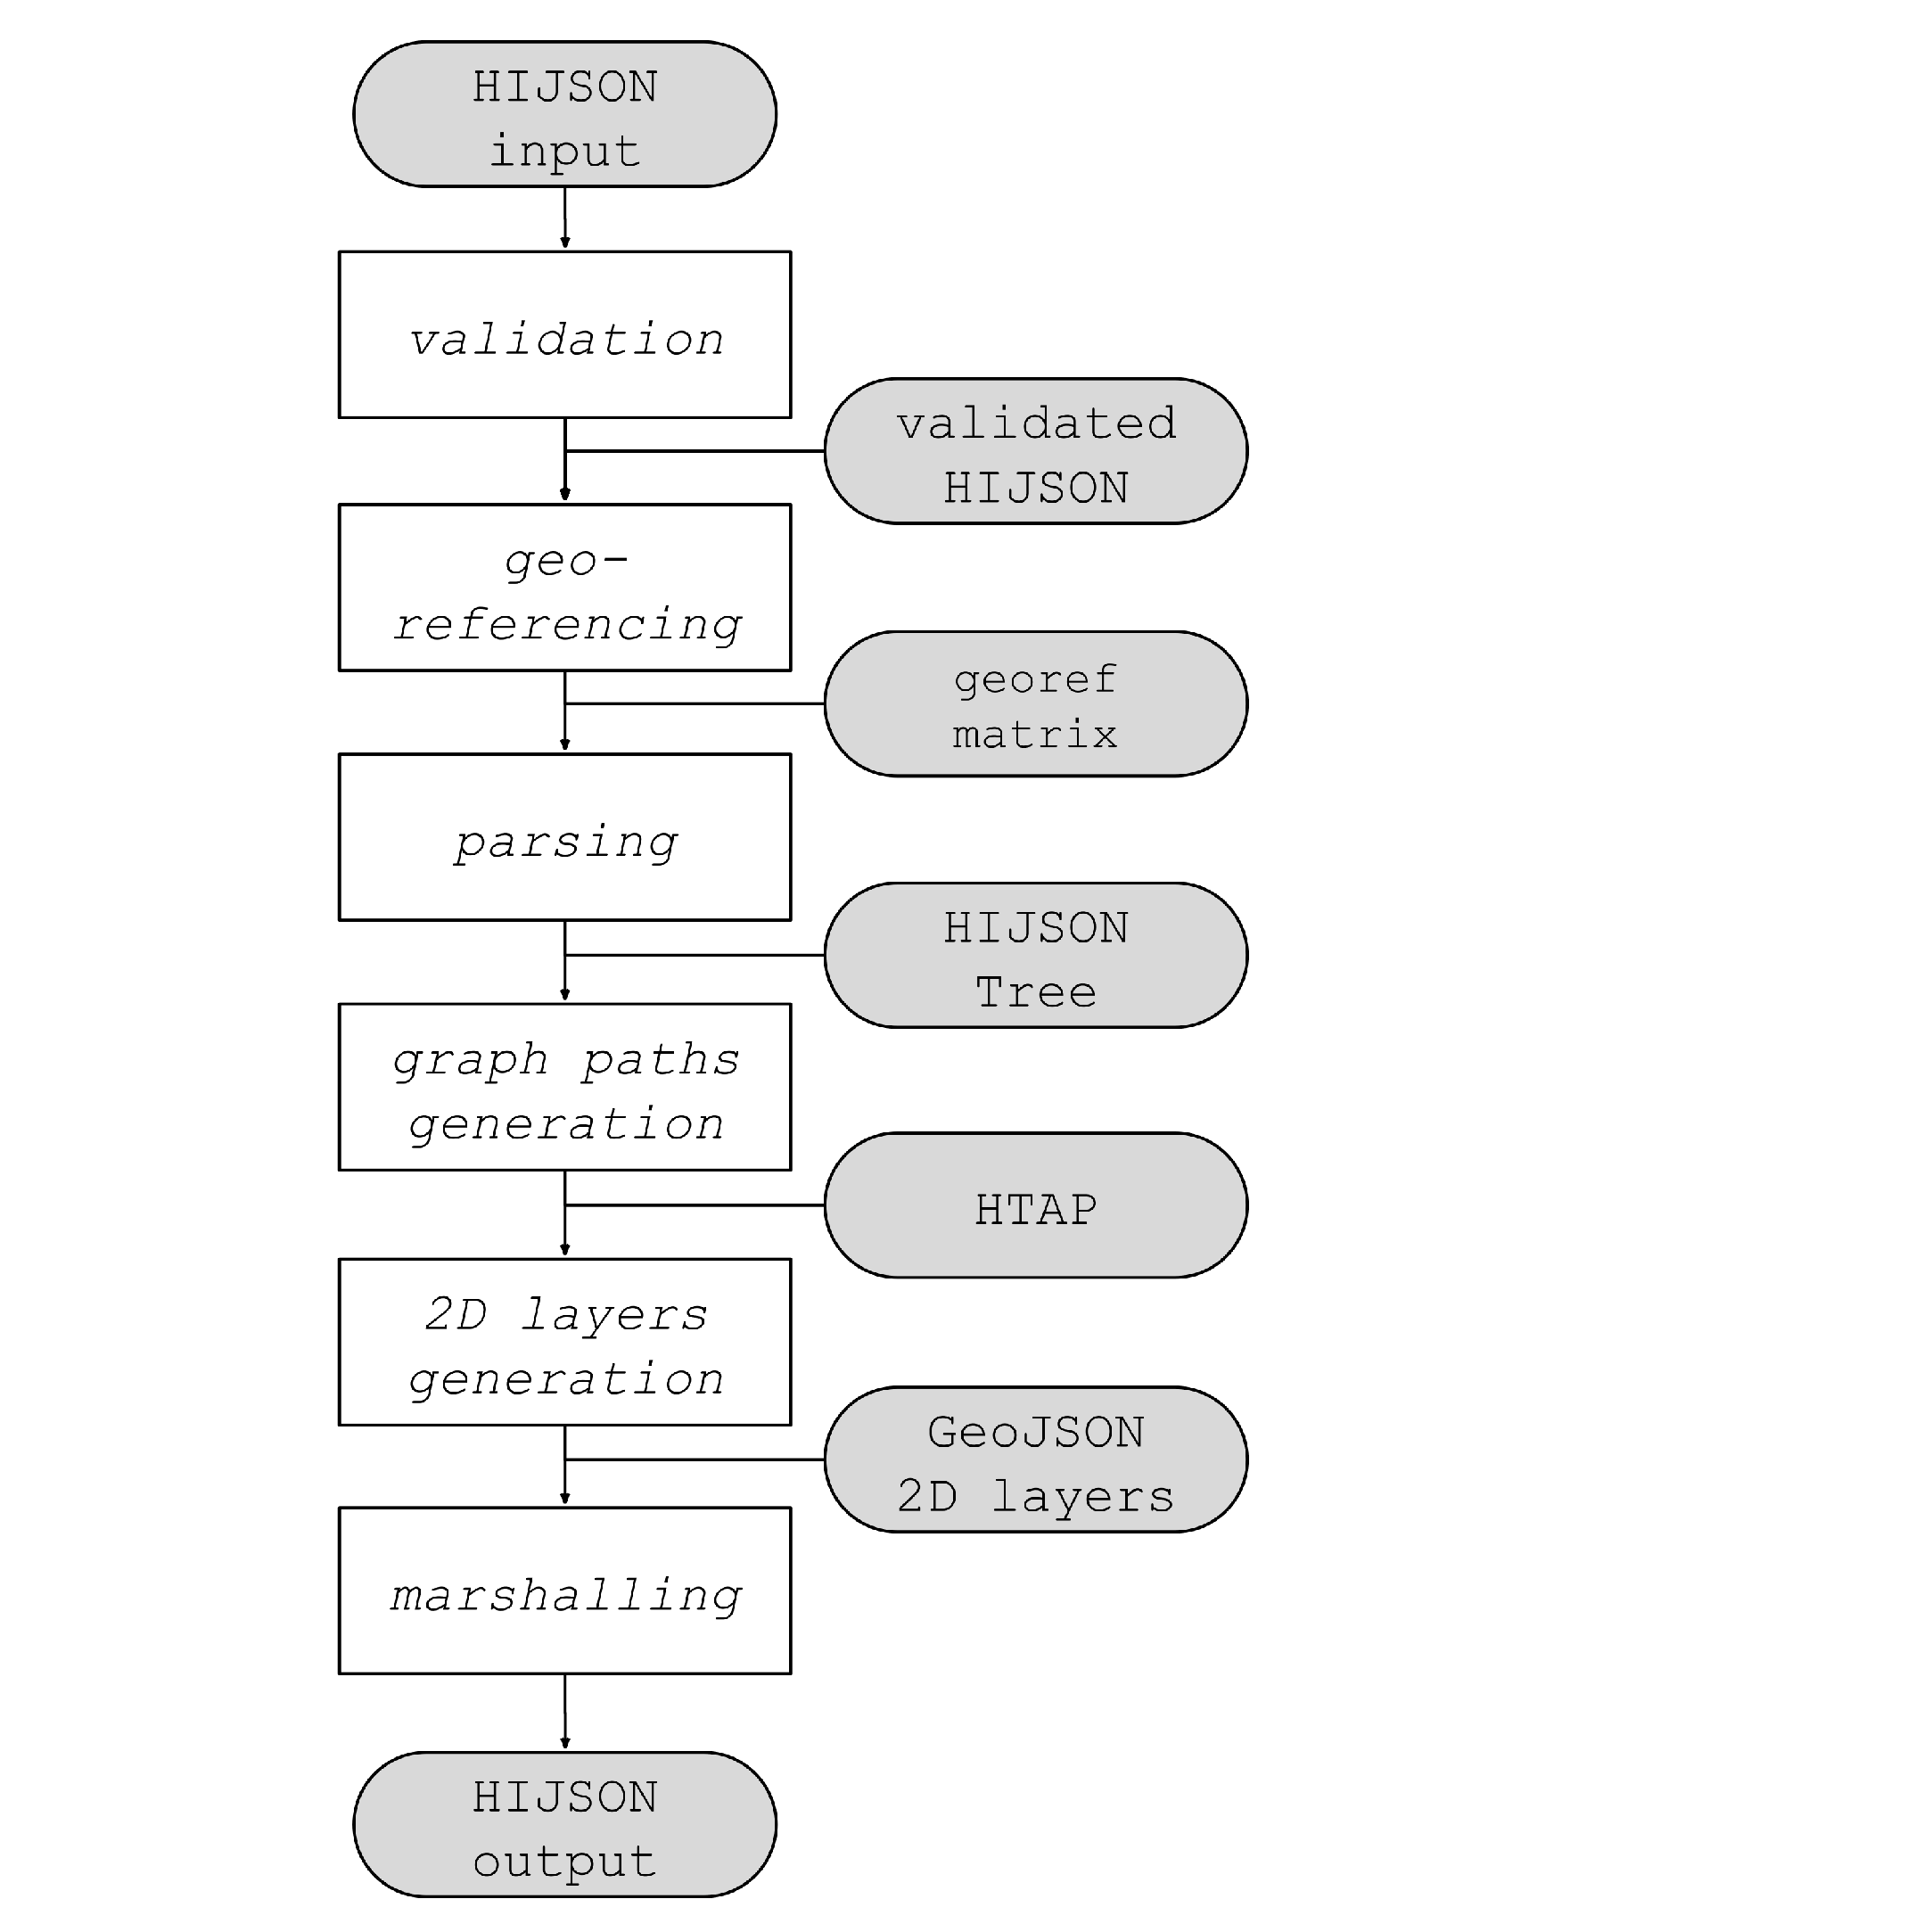
\epsfig{file=images/pipeline.eps, height=0.4\textwidth}
\caption{``HIJSON processing pipeline''}
\label{fig:pipeline}
\end{figure}

\begin{enumerate}
\def\labelenumi{\arabic{enumi}.}
\itemsep1pt\parskip0pt\parsep0pt
\item
 \textit{\texttt{validation}} - The first one is the validation stage. In
 order to begin with the effective transformations the input HIJSON
 document must be compliant with the rules defined in (AGGIUNGERE REF
 TO PARAGRAFO REGOLE DI VALIDITA'). In the case the validation stage
 fails, processing aborts and do not continue to following stages. If
 the stage success, the output for the next stage is a validated
 HIJSON.
\item
 \textit{\texttt{georeferencing}} - In the second stage, in order to allow
 for continuous outdoor/indoor navigation, the system needs to compute
 the georeferencing matrix, a linear operator able to transform local
 coordinates into global coordinates (referred to world coordinate
 system as latitude and longitude misures) and viceversa. This task is
 accomplished by solving a linear system obtained from information
 contained in HIJSON configuration part and precisely from the
 correnspondance of three real word points to three points included
 into the HIJSON document.
\item
 \textit{\texttt{parsing}} - The parsing stage, takes the validated and
 georeferenced HIJSON as its input, that as illustrated before can be
 thought of as a list of HIJSON Elments, parses them and produce an
 istance of HIJSON Tree. The HIJSON Tree is an object in memory
 representing the tree hierarchical structure of the building described
 by the HIJSON document.
\item
 \textit{\texttt{graph paths generation}} - The fourth stage is in charge
 of the generation of the graph paths. This aim is accomplished
 according to the algorithm described in (AGGIUNGERE RIFERIMENTO A
 \#\#\#\# Automatic generation of valid paths). The graph paths will be
 useful afterwards to coumpute valid paths from couple of point of
 interest on the graph. Once the graph paths has been computed, the
 input HIJSON Tree is augmented with paths information, becoming what
 has been called an HTAP (HIJSON Tree Augmented with Paths).
 Augmentation always takes place as leaf nodes added as children of a
 specific (e.g. ``room'') level.
\item
 \textit{\texttt{2D layers generation}} - The fifth stage is the
 generation of GeoJSON layer. For each level, the system generates one
 geoJSON layer that will be use for the creation of 2D map. Each layer
 contains the children of `level' node in the HIJSON Tree. Every class
 contains a boolean value that is used to choose which class will be a
 part of geoJSON layer. Every element has a geographical coordinates
 calculated by the transformation matrix with regard to the local
 coordinates of the HIJSON element.
\item
 \textit{\texttt{marshalling}} - The last stage is responsible of execute
 a serialization of the the transformed data. Tasks like breaking
 dependency-loops and stringification are performed. This stage is
 useful mainly serverside, as and the output is stored ready to be
 served to any requiring client.
\end{enumerate}

\subsubsection{Algorithmics: automatic generation of valid paths}\label{algorithmics-automatic-generation-of-valid-paths}

The fourth stage of the processing pipeline is responsible for the
generation of a graph of valid paths through the entire model
represented by the intput HIJSON document. The graph generated according
to the algorithm described in the following, although not optimal,
ensures a complete coverage of the surface while limiting the numebr of
generated nodes. Resulting graph is weigthed on the edges with nodes
distances and each node represents alternatively:

\begin{enumerate}
\def\labelenumi{\alph{enumi}.}
\itemsep1pt\parskip0pt\parsep0pt
\item
 standard path node, i.e.~a junction node or possibly an endpoint of a
 path;
\item
 connection node, used as subproblem composing element in the divide et
 impera approch adopted (as described below).
\item
 element nodes ie. HIJSON Element (whose HIJSON Class explicitly grants
 his presence in the graph), typically an endpoint of a path;
\end{enumerate}

Such a graph allows for directions calculations between any two given
nodes. Although different approaches have been explored \cite{6999103}, 
a very classical solution has been selected in this case, so directions 
are actually computed clientside applying the Dijkstra's shortes route 
algorithm on the graph. 

Taking advantage of the hierarchical structure of the HIJSON document,
and according to the divide et impera approach, the problem of the graph
paths generation is splitted in several sub-problems which consist in
the computation of the sub-graphs relative to each room, or more
generally ambience. The sub-graphs are then linked together through the
connection nodes (which in most cases represents doors). The resolution
of each sub-problem (as depicted in figure METTERE RIFERIMENTO ALLA
FIGURA), is composed by 4 phases:

\begin{enumerate}
\def\labelenumi{\arabic{enumi}.}
\itemsep1pt\parskip0pt\parsep0pt
\item
 Computation of the walkable area of the ambience: this task is
 accomplished subtracting area of the possibly encumbrances to the area
 of the ambience; the result is tipically a surface with holes;
\item
 Triangulation of the walkable area: the computed surface is
 triangulated taking into account the presence of holes;
\item
 Identification of graph nodes: for each triangle side completely
 internal to the area, its midpoint is selected as standard path node;
\item
 Junction of nodes: nodes relative to the same triangle are then linked
 together; both element nodes and connection nodes (i.e.~doors) are
 linked to the nearest node in the ambience (i.e.~room).
\end{enumerate}

\begin{figure*}[!htbp]
 \centering
 \begin{subfigure}[b]{0.235\textwidth}
 \includegraphics[width=\textwidth]{images/graph-generation/single/graph-generation-1}
 \caption{}
 \label{fig:graph-generation-a}
 \end{subfigure}
 ~
 \begin{subfigure}[b]{0.235\textwidth}
 \includegraphics[width=\textwidth]{images/graph-generation/single/graph-generation-2}
 \caption{}
 \label{fig:graph-generation-b}
 \end{subfigure}
 ~
 \begin{subfigure}[b]{0.235\textwidth}
 \includegraphics[width=\textwidth]{images/graph-generation/single/graph-generation-3}
 \caption{}
 \label{fig:graph-generation-c}
 \end{subfigure}
 ~
 \begin{subfigure}[b]{0.235\textwidth}
 \includegraphics[width=\textwidth]{images/graph-generation/single/graph-generation-4}
 \caption{}
 \label{fig:graph-generation-d}
 \end{subfigure}
 
 \caption{Graph paths generation: 
 (a) detection of obstacles and computation of walkable area; 
 (b) triangulation of walkable area; 
 (c) identification of graph nodes area; 
 (d) junction of nodes.
 }
 \label{fig:graph-generation}
\end{figure*}

\subsection{HIJSON Class definition}\label{hijson-class-definition}

To exploit the possibilities offered by HIJSON Toolkit, along with the
HIJSON document, some custom dynamic behaviours must be described. These
behaviours encapsulate the specificities relative to comminucation
procols with the sensors as well as user interaction peculirities. The
interface for these behaviours is the HIJSON Class.

\begin{figure}[!h]
\centering
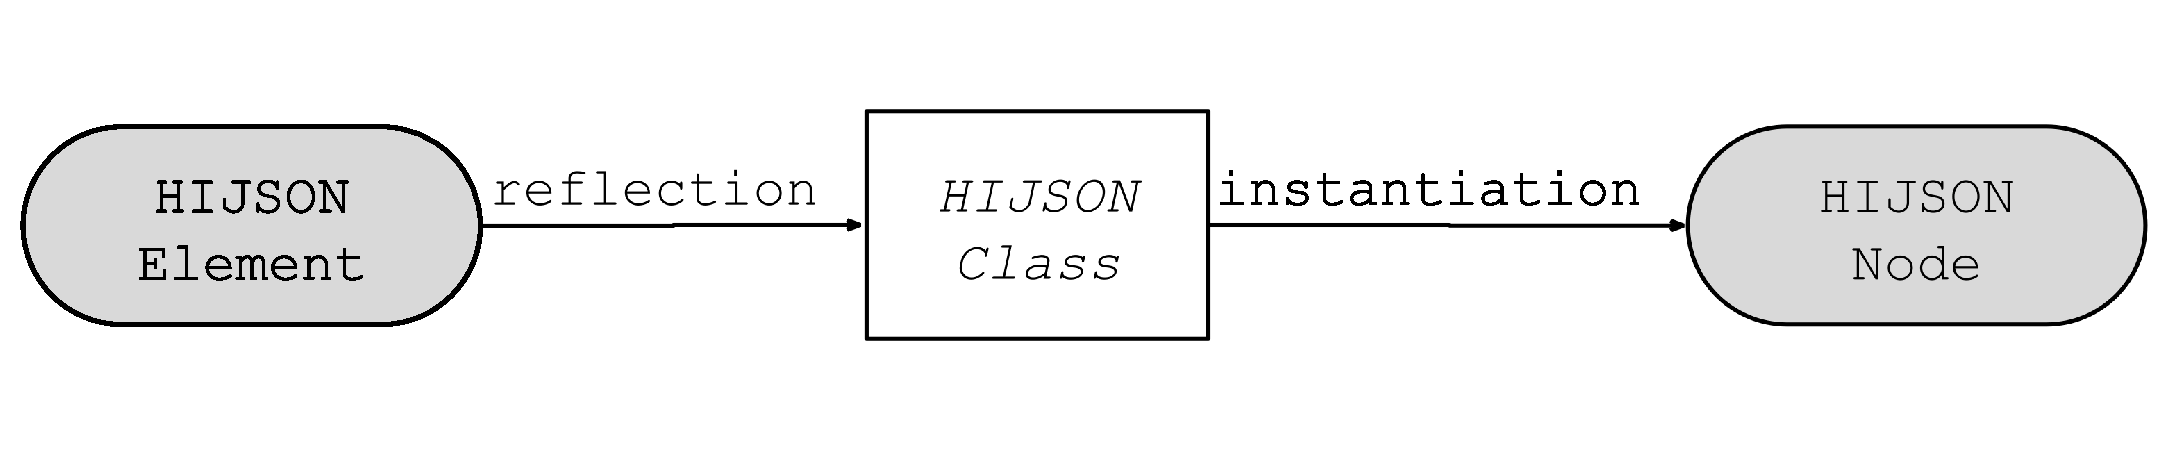
\epsfig{file=images/element-class-node.eps, width=0.44\textwidth}
\caption{``HIJSON Element/Class/Node relashionship''}
\label{fig:elem-class-node-rel}
\end{figure}

Each HIJSON Element of the HJSON document given as input, has a dynamic
counterpart, a running instance called HIJSON Node, instantiated
according to the corresponding HIJSON Class via relfection methods (see
picture XXXXX).

To specify a new HIJSON Class means to extend the Toolkit to deal with a
new class of HIJSON Element.

To extend the toolkit to deal with a new class of HIJSON Element is
required to to specify a new HIJSON Class, defining the following
properties and methods:

\begin{itemize}
\item
 \texttt{in\_graph}: a boolean value to express if the element is an
 approachable point in the graph paths;
\item
 \texttt{in\_2D\_map}: a boolean value to express if the element is
 wanted in the 2D map;
\item
 \texttt{get2DStyle}: a method that returns the 2D map appearence of
 the element, essentially HTML and CSS code;
\item
 \texttt{get3DModel}: a method that returns the 3D model appearence of
 the element, a \emph{THREE.js Object3D};
\item
 \texttt{getWidget}: a method that returns the information widget, a
 \emph{React} component;
\item
 \texttt{getProxy}: a method that returns server side proxy which
 encapsulate IoT sensor communication protocol, a \emph{Node.js
 module}.
\end{itemize}

User's needs for new indoor elements, different sensor equipment,
alternative representation on 2D or 3D viewport are accepted by the
definition of new HIJSON Classes that allows in this way single point
custom extension of the Toolkit capabilities.


\begin{figure*}[htb]
\centering
\includegraphics[width=\textwidth]{images/web-framework.png}
\caption{``HIJSON Web Framework UI''}
\label{fig:web-framework-ui}
\end{figure*}


\section{HJSON Web Framework}\label{hjson-web-framework}

The HJSON Web Framework responds to the needs of an extendable,
customizable, and scalable framework which provides at the same time IoT
monitoring, realtime multi-person tracking and crossfloor user
navigation.

Expandability and customizability derives from both design choises and
HIJSON inherent characteristics, the possibility of semantic extensions.
Scalablility is directly borrowed from technologies used for the
software development: \emph{JavaScript} language, using \emph{Node.js},
in particular \emph{Express.js} as backend framework, exploiting the
power of WebSocket protocol through the \emph{Socket.io} library.

Being supported by the web as bearing platform, the framework exposes
also an highly availability: it is so simple to use as to visit a
website, both from desktop or mobile devices, without explicit
requirements to install any software from proprietary stores (access to
which is often denied from business devices).

The HIJSON Web Framework deeply relies on HIJSON Toolkit and offers the
overal client/server architecture and a convinient, highly intractive
user interface, leaving aside the specific indoor positioning system and
the IoT sensors, to deal with a robust interface is provided and
described in the following seciton.

\subsection{Applications}\label{applications}

The Framework has been designed focus on two different possible kind of
users: the \emph{Explorer} and the \emph{Supervisor}. They have
different requirements and are likely equipped with different devices:
while the \emph{Supervisor} monitors the indoor environment through a
desktop workstation, the \emph{Explorer} has a smartphone available and
needs to be routed across the building.

\begin{figure*}[htb]
\centering
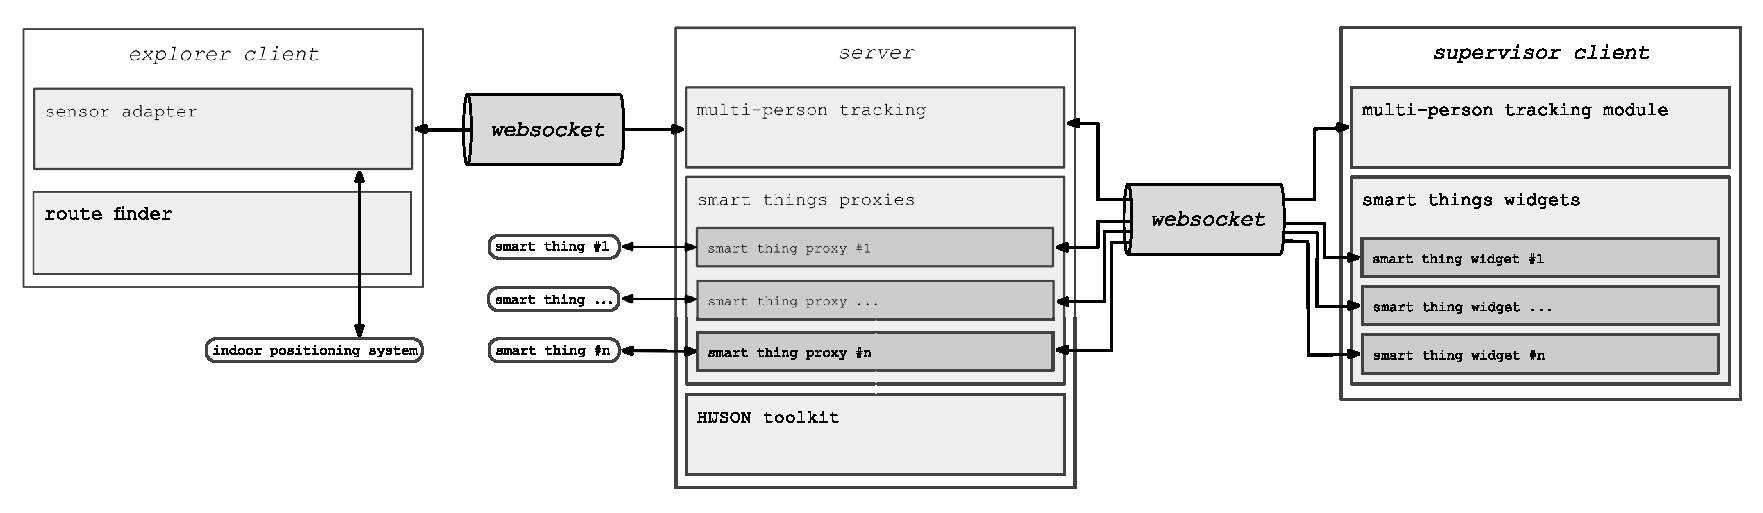
\epsfig{file=images/architecture.eps, width=\textwidth}
\caption{``HIJSON Web Toolkit architecture''}
\label{fig:pipeline}
\end{figure*}


\subsubsection{IoT monitoring}\label{iot-monitoring}

Every element in the HIJSON environment is capable of showing information
about itself, so it can be analyzed by the user. The modularity of the HIJSON
Toolkit permits to show particular information or UI about a specific object,
using polymorphic behaviours of the different HIJSON Nodes. If an object is
connected to the network and it is capable of interaction, the user can
benefit of its functions through the system (e.g. if the object is a
thermostat, the user can see the temperature in the room and can turn on/off
the heating). If the object isn't interactive, the system can show static
information (e.g. for fire Extinguisher, the system shows the last date of
checking).

\subsubsection{Realtime multi-person tracking}\label{realtime-multi-person-tracking}

A typical task performed by a \emph{Supervisor} can be the monitoring of users
locations inside the building. This operation can be required for various
reasons, e.g. security or logistics. The devices that equips the
\emph{Explorers} can be used to track their position in realtime, giving the
\emph{Supervisors} the whole picture of the presences inside the building in
every moment.

\subsubsection{Crossfloor user navigation}\label{crossfloor-user-navigation}

As shown in the algorithmics section, the HIJSON Toolkit provides a particular
strategy to assemlbe a graph of possible paths inside the building. This
graph, represented also in the form of a weighted adjacency matrix, can be
easely used to compute paths between two nodes inside the building. To
achieve this result, the matrix, which edges are weighted according to the
distance between two nodes, is used as input in an applicaiton of the
Dijkstra's algorithm. The result is the shortest path between two selected
nodes of the graph. Thanks to the crossfloor connections of nodes
representing stairs or elevators, the paths calculated can also start and end
on different stories.



\subsection{Architecture}\label{architecture}

Like the vast majority of the web based application, the Framework exposes an
overall architecture that is inherently \emph{client/server}. In particular,
two different type of possible client are identifiable: the \emph{Supervisor}
client and the \emph{Explorer} client. Both of them connect to the same
server.

The indoor space described by the HIJSON document provided as input is
processed by the server (cfr. PROCESSING PIPELINE). After that any connecting
\emph{Explorer} client, presumably through a mobile device, will be provided
with the information to perform crossfloor navigation of the building, while
reporting user position to the server. The server will feed any connecting
\emph{Supervisor} client with users positions, along with data from sensor-
equipped things present in the environment, realizing the IoT monitoring and
the realtime multi-person tracking.

\subsubsection{Server Architecture}\label{server-architecture}

The architecture of the server is depicted in XXXX. A web server module
is responsible for listenning to connecting clients. Each client
connection is handled by the web server module providing all the
required resources and opening one websocket channel, through which will
flow \emph{Explorer} and/or \emph{Supervisor} communication protocol
data. In particular, \texttt{multi-person\ tracking} module receives
position data from \emph{Explorer} clients. It aggregates and sends
these information to connected \emph{Supervisor} clients through the
websocket channel, using a simple but realible protocol later described.
Indipendence from particular IoT sensor equipment communication protocol
is achieved by the \texttt{smart\ things\ proxies} module through the
proxies modules obtained by the HIJSON Class definition
(\texttt{getProxy} method previuosly described).

\subsubsection{Explorer client architecture}\label{explorer-client-architecture}

The \emph{Explorer} client architecture is generally deployed on a
mobile device, usually supplied to a user who needs to be routed across
the environment described by HIJSON document. The
\texttt{sensor\ adapter} module encapsulates the communication logic
with the indoor positioning system. The presence of this module ensures
indipendece from particularly tecnology allowing client \emph{Explorer}
to rely on different indoor positioning systems: INDICARE ESEMPI SENSATI
E CUTTING EDGE DI POSIZIONAMENTO INDOOR. INTRODURRE IL PROBLEMA DELLA
COMUNICAZIONE A LIVELLO API DEL BROWSER CON SENSORISTICA PER LA
RILEVAZIONE DELLA POSIZIONE.

Every time the \texttt{sensor\ adapter} observe a perceptible
modification in user position sends the new position information to the
server through the single opened websocket, using the a message with the
following syntax:

\begin{verbatim}
currentPosition = {
 coordinates: [x, y],
 levelId: level-ID 
}
\end{verbatim}

Relevant information includes, beside current coordinates, the
indication of the story of the possibly multilevel building the user is
in. The \texttt{smart\ things\ widgets} module being in common with the
client \emph{Supervisor}, has been treated in the next section.

\subsubsection{Supervisor client architecture}\label{supervisor-client-architecture}

The Client \emph{Supervisor} architecture shows two modules. The first
one, the \texttt{multi-person\ tracking} module, is responsible to
receive through the websocket, from the server information about
explorers of the environment, showing them in the user interface. The
second module, the \texttt{smart\ things\ widget} communicates with the
server to propose to the user realtime information about sensor-equipped
objects in the environment. Data passes through the single websocket
opened between the server and every \emph{Supervisor} Client. Rely on a
naive but effective communication protocol, each smart thing widget
exchaange data only with respective smart thing proxy on the server. To
ensure the the data is sent only when the user requires the information
relative to a specific smart thing, a widget lifecycle protocol is
implemented: it is based on the 4 events \texttt{on\_before\_show},
\texttt{on\_show}, \texttt{on\_before\_hide}, \texttt{on\_hide}
triggered, as suggested by their names when a widget is shown or hidden.
When the user requires information about a smart thing, its widget has
to be rendered, but \texttt{on\_before\_show} the server is notified to
connect via relative proxy to the sensor. Once connected, the server
begin to send data via webscocket. Received data is shown through the
wodget to the user. When done, or \texttt{on\_before\_hide} event of the
widget, a notification is sent to the server announcing to stop sending
data and the proxy close the connection to the sensor. Widget lifecycle
protocol ensures that only requiring data is sent from th eserver to the
client.


\section{Case study}\label{use-case}

As the first case study has been taken into account the need of SoGeI to support its data center maintaince, which is subject to strict access control policies. 
Lo scenario considerato consiste nell'intervanto di manutenzione da parte di un operatore che deve muoversi nell'ambiente e localizzare all'interno di un datacenter dalle enormi dimensioni la macchina su cui operare, individuandolo tra migliaia di rack di aspetto simile. Tale operatore sarà quindi equipaggiato con un client explorer. Il client explorer guiderà l'operatore fino al sottosistema su cui intervenire, notificandone al contempo la posizione ad ogni istante.

Le figure responsabili, attraverso il supervisor client possono monitorare la situazione degli smart object, che in questo caso spaziano dalle webcam ai sistemi di allarme antincendio ma comprendono anche le macchine fische, sicchè sia possibile monitorarne lo stato di funzionamento, temperatura di esercizio e carico di lavoro...


The real­time awareness of the relative positions between
the ‘maintenance man' andthe rack ­ containing the machine­ will help us
increasing safety and reducing intervention times.
Infatti, le figure responsabili, con diritti di accesso al client supervisor, avranno quindi modo di monitorare le posizione degli operatori attivi all'interno del datacenter verificando che essi non devino su percorsi non autorizzati.

In particolare tali supervisori, nello scenario di manutenzione in analisi, tracciando l'intervento dell'operatore in tempo reale possono scaricare il sistema target della manutenzione da tutti i servizi che offre, migrando le corrsipondenti macchine virtuali e distribuendole su altri sistemi, garantendo così continuità di servizio e diminuendo il global risk factor. Terminato l'intervento tecnico, lo stato precedente può essere ripristinato. 




%----------------------------------------------------------------------------

% right sub­system (inside the rightrack among thousands). We will call them the
% ‘maintenance man’. The real­time awareness of the relative positions between
% the ‘maintenance man' andthe rack ­ containing the sub­system ­ will help us
% reducing intervention times and increasing safety. If you knew when the
% maintenance process starts, you couldautomatically move,in real time,
% services, that is virtual machines, to other systems,thus
% maintainingcontinuity of services and, in the same time, reducing the
% globalrisk factor. Whenmaintenance is over, and the technician moves away, you
% couldinstantly restore thepre­existing conditions of services, that is,
% immediately after havingperformed an outright test.

% We are now trying to
% verify the possibility to perform a realtime control over the maintenance
% workflow in a complex Data Center. 

% Inparticular, wehave to support the process of those in charge of carrying out
% the ticket­maintenance reaching, as quick as possible and without error, the
% right sub­system (inside the rightrack among thousands). We will call them the
% ‘maintenance man’. The real­time awareness of the relative positions between
% the ‘maintenance man' andthe rack ­ containing the sub­system ­ will help us
% reducing intervention times and increasing safety. If you knew when the
% maintenance process starts, you couldautomatically move,in real time,
% services, that is virtual machines, to other systems,thus
% maintainingcontinuity of services and, in the same time, reducing the
% globalrisk factor. Whenmaintenance is over, and the technician moves away, you
% couldinstantly restore thepre­existing conditions of services, that is,
% immediately after havingperformed anoutright test.



\section{Conclusions}\label{conclusions}

In this paper a novel format for indoor cartographical description has been
introduced, named HIJSON. Utilization of local metric coordinate system,
avoiding the manipulation of geographical coordinate really inconvenient when
dealing with indoor spaces and objects, greatly simplify the drawing up
process of the document. Process that can be further improved realizing a
graphical editor to assist the user during the description of the indoor
space. The implementation of such an editor is already programmed.

The HIJSON format focuses on a hierarchical representation of the indoor
spaces that allows for completely capturing their topology. On the basis of
this representation a virtual web environment can be rebuilt working as a
unifying platform to run a bunch of different applications. The reference
architecture of such a platform has been also implemented and described in
this work. The architecture supports a range of applications: IoT monitoring,
realtime-multiperson tracking and user cross-storey navigation are already
implemented and described. A very convenient way to extend representation
capabilities of smart objects is also mentioned as semantic extensions. These
extensions (which affects both document format and web framework) might be
easly collected in a public repository. Community could both use public
available extensions or contribute by mapping new (smart) objects inside the
HIJSON document.


%
% The following two commands are all you need in the
% initial runs of your .tex file to
% produce the bibliography for the citations in your paper.
\bibliographystyle{abbrv}
\bibliography{doceng2015.bib}  % sigproc.bib is the name of the Bibliography in this case
% You must have a proper ".bib" file
%  and remember to run:
% latex bibtex latex latex
% to resolve all references
%
% ACM needs 'a single self-contained file'!
%

\end{document}
